\subsection{Column Image Transformer}
    
    The Column Image Transformer (CIT) is the first transformer-based model approach in this thesis. It processes input data in a columnar format as examined in the previous section in more detail see \autoref{sec:IntroColumnModel}.


    \begin{figure}[H]
        \centering
        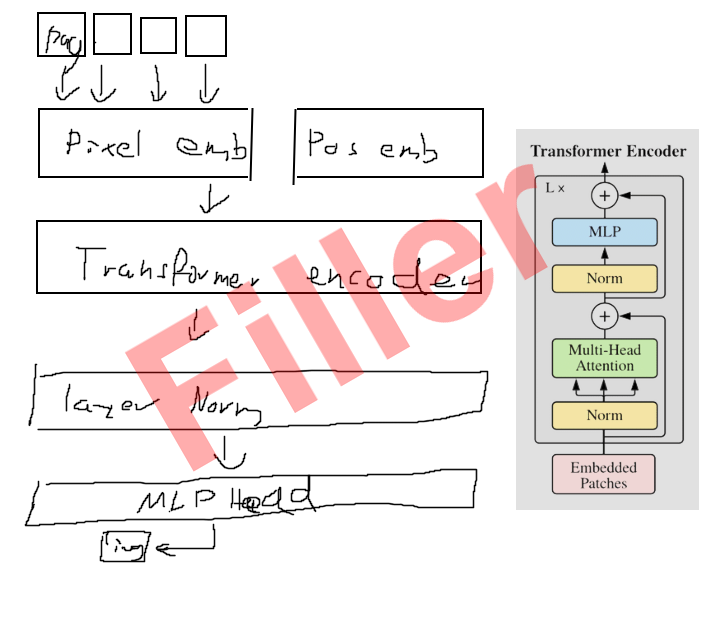
\includegraphics[width=0.8\textwidth]{imgs/CITModel.png}
        \caption{Column Image Transformer Model}
        \label{fig:ColumnImageTransformer}
    \end{figure}

    The image above shows the steps carried out by the CIT model. The input data is reshaped into a columnar format, which is then embedded into a higher-dimensional space. The positional embedding layer adds positional context to the input data. The transformer layer processes the data, and the output is then transformed back into a columnar format. After going through a final layer normalization and another MLP that converts back from the embedded layer to 3 colors, the model is trained using a Mean Squared Error (MSE) loss function.


    %TODO: Add more information and a illustration
    This section will go more into detail about the steps form the [Data loader -> Pixel Embedding -> Positional Embedding -> transformer layer -> Pixel Emb ->  Loss calculation and evaluation].

    \subsubsection{Get Data as Columns}

    The data is loaded into a DataLoader object as described in \autoref{sec:DataHandling} and iterated over to extract it as a 4-dimensional tensor (Batch, Color Channels, Height, Width). This data is reshaped into a columnar format, resulting in two tensors: the \(source\) and \(targets\), both with the shape (Batch, Height, Color Channels). The target tensor is shifted one pixel downwards to the prediction of subsequent pixels by the model. This reshaping and shifting method is commonly employed in transformer-style learning because it enables the model to process data more efficiently in terms of computational speed and resource utilization. The source tensor is then fed into the model, and its output is compared against the targets using the Mean Squared Error (MSE) loss function.

\begin{figure}[H]
\centering
\begin{lstlisting}[language=Python]
# data: (Batch, Color, Height, Width)
def get_batch(data):

    source = data[:, :BLOCK_SIZE, :BATCH_SIZE]
    targets = data[:, 1:BLOCK_SIZE+1, :BATCH_SIZE]

    source = rearrange(source, 'c h b -> b h c')
    targets = rearrange(targets, 'c h b -> b h c')

    return source, targets
\end{lstlisting}
\caption{Python function to convert data into a columnar format}
\label{fig:get_batch_CIT}
\end{figure}

    \subsubsection{Pixel Embedding}

    The \(source\) data is embedded into a higher-dimensional space using pixel embedding layers. This MLP is a straightforward linear layer that maps the input data to a higher-dimensional space, transitioning from \(3\) color channels to \(N_{\text{EMBD}}\). This layer consists of a linear transformation followed by a ReLU activation function and is succeeded by a dropout layer.

    Through testing and experimentation, it seems that the optimal configuration for the pixel embedding layer involves a sequence of dimensionality increases. The most effective pathway identified begins by scaling the dimensionality of the input from the original image channels \(C\) to one-fifth of \(N_{\text{EMBD}}\) (\(\frac{1}{5}N_{\text{EMBD}}\)), then increasing it to one-half of \(N_{\text{EMBD}}\) (\(\frac{1}{2}N_{\text{EMBD}}\)) until reaching \(N_{\text{EMBD}}\). The pixel embedding layer is followed by a dropout layer with a dropout rate of 0.2.

    %TODO:
    Todo: Add Code or Image of the Pixel Embedding Layer

    It is crucial to highlight the importance of not using a layer normalization (layernorm) layer in the initial few layers of the model. Incorporating a layernorm layer too early results in outputs that are predominantly black and white. This phenomenon occurs because the color channels \(C\), which are comprised of Red, Green, and Blue, are normalized by the layernorm layer to exhibit uniform values across these channels. As a consequence, this normalization process hinders the model's ability to learn the distinct colors of the pixels, relegating it to only wrong grayscale variations.

    \subsubsection{Positional Embedding}
    \label{sec:CIT_PositionalEmbedding}

    The positional embedding layer in this model utilizes a learnable embedding matrix of size \text{BLOCK\_SIZE} times \(N_{\text{EMBD}}\), where \text{BLOCK\_SIZE} represents the context length, or the height of an image. This layer operates by assigning each position within this vertical context a unique embedding vector, thereby mapping the original pixel positions to a high-dimensional space characterized by \(N_{\text{EMBD}}\) dimensions. The integration of these positional embeddings is achieved through their direct addition to the output of the pixel embeddings, effectively enhancing the model's ability to maintain positional awareness across the image height.


\begin{figure}[H]
    \centering
    \begin{lstlisting}[language=Python]
class ColumnTransformer(nn.Module):

    self.position_embedding_table = nn.Embedding(BLOCK_SIZE, N_EMBD)
    #[...]

def forward(self, idx, targets=None):

    # tok_emb: (B, H, N_EMBD)
    tok_emb = self.pixel_embedding(source) 

    # pos_emb: (H, N_EMBD)
    pos_emb = self.position_embedding_table(torch.arange(H)) 

    # x: (B,H,N_EMBD)
    x = tok_emb + pos_emb 
    #[...]
\end{lstlisting}
\caption{Python code snippet for the Positional Embedding Layer}
\label{fig:posEmbend_CIT}
\end{figure}
   
    \subsubsection{Transformer Layer}
    \label{sec:transformer_CIT}

    The Transformer layer forms the core of the model's architecture and is crucial for processing the data. It utilizes self-attention mechanisms \autocite{vaswani2023attention} to weigh the importance of different pixels relative to each other, allowing the model to focus on relevant parts of the input when predicting the next pixel in a column. 

    In this model, each Transformer layer receives the input from the previous layer. The layer then processes this input using a multi-head attention mechanism, which allows the model to capture various aspects of the input at different positions simultaneously. This is followed by a series of normalization and feed-forward layers. All are combined into a block that is repeated multiple times. See \autoref{sec:transformer_layer_Python} for the code snippet.


    \subsubsection{Output Layer}

    The output layer is like the pixel embedding a simple MLP that converts the data back to the original color space. It has the same structure but reversed like the Pixel Embedding layer but with the output dimensionality set to \(3\), representing the Red, Green, and Blue color channels. After the shrinkage of the dimensionality, the output is passed through one final sigmoid to map the resulting colors to 0-1.

    \subsubsection{Sigmoid Compared to Clamp}
    \label{sec:sigmoid_vs_clamp}
    
    Due to discoloration issues in the model output, the performance has been evaluated using two different activation functions: sigmoid and linear clamp. Typically, the sigmoid function maps input values to a range between 0 and 1. However, in the context of color values, this compression into the [0, 1] range can prevent achieving true black and white colors, as extremely large or small inputs are needed to reach the extremes of 0 or 1. Initially, the linear clamp function, which restricts input values to a specified range without compression, seemed to better preserve the distinct black and white colors. However, it has several notable disadvantages, such as ...(please fill in the biggest problem with backpropagation).
    
    %TODO:
    TODO: Add more information about the Problem with the clamp function

    In discussions about this problem, it was suggested that the lack of training data featuring significant black and white samples might be a contributing factor. After collecting more data and expanding the training set, the issue was resolved, and the model performance with the sigmoid activation function is very similar, showing improvement comparable to the clamp function.
    
    \subsubsection{Discoloration in the Model Output}
    
    The model faces similar discoloration issues as mentioned in section \autoref{sec:sigmoid_vs_clamp} with certain colors. When the model starts with a random pixel, it often struggles to consistently generate the intended pattern in that color or starting pattern. Some evidence suggests that the training set may be too small, as the issue was less noticeable with a larger dataset. Generally, transformers require significantly more data to improve performance \autocite{chen2022dearkd}. However, this problem has not yet been resolved, and further research is needed.

    \subsubsection{Classification or Regression}
    \label{sec:ClassificationOrRegression}

    To see if the method (Classification / Regression) has a big impact on the performance of the model both methods are tested. For comparison grayscale input and outputs are used. This strategy is particularly advantageous because it minimizes the complexity arising from the vast number of potential output possibilities in classification tasks. With RGB color representation, each pixel can be classified into one of 16,581,375 distinct color combinations (255 possibilities for each of the Red, Green, and Blue channels).

    Utilizing grayscale input and outputs, simplifies the classification task, reducing the number of potential outcomes to a manageable range. Grayscale images, with their single intensity channel representing luminance, offer a more straightforward basis for analysis. This simplification allows for a more focused evaluation and a faster check if the model performs differently or better.

    %TODO:
    TODO: Add more information about the Classification and Regression Results
        

    \subsubsection{Training the Model}

    The training process starts by selecting the hyperparameters and arguments for the model. To test the basic functionality of the model, the training process is kept simple, and they are trained on a single GPU. Most of the training is done via the Slurm cluster, which uses a batch script to configure the hardware and training parameters. All the parameters can be found in detail in the appendix \autoref{sec:trained_models_hyperparameters}.
    
    

    2.3.5 Training Protocols
    Discuss the training process, highlighting any unique considerations for the spiral data format.

    \subsubsection{Experimental Results}
    
    Multiple experiments are conducted to evaluate the performance of the CIT model. The experiments are designed to test the models ability to generate images, the quality of the generated images, and the models performance on different datasets. The results are analyzed to identify the strengths and weaknesses of the model.

    \begin{itemize}
        \item \textbf{Color test:} To test the models capability to generate certain colors the model is given a test image with one single color filling the whole context. Then the model generates the next flowing 32 pixels. 
        
        %TODO: 
        TODO: Add color test images models output

        \item \textbf{Zebra pattern test:} The second test is to see if the model is capable of generating a zebra pattern. The model is given a vertical and a horizontal test image with a black and white colored zebra pattern with a pixel width of 3. The model then generates the next 32 pixels.
        
        %TODO:
        TODO: Add zebra pattern test images models output
        

        \item \textbf{Classification test:} The third test is to see if the model performs equally well as classification model as a regression model. The model is trained on grayscale images and outputs grayscale images. More information can be found in \autoref{sec:ClassificationOrRegression}.
        
        %TODO:
        TODO: Add classification test images models output
        

    \end{itemize}

    \subsubsection{Challenges and Limitations}
    2.3.9 Identified Challenges
    Discuss specific challenges encountered during the development and implementation phases.

    2.3.10 Limitations of the Spiral Transformer
    Critically analyze the limitations and potential drawbacks of using a spiral approach.
